\section{Background}\label{sec:background}

\subsection{MAPF}\label{sec:background_mapf}

The following definitions of Multi-Agent Path Finding (MAPF) follow the ones in~\cite{husvobbass22a}. MAPF is a triple $(V,E,A)$ where \(V,E\) denotes a connected graph, \(V\) being a set of vertices and \(E\) a set of edges connecting them. Then \(A\) being a set of agents. For each agent \(a=(s,g) \in A\), \(s\) is a vertex in \(V\) denoting the starting location and \(g\) is also a vertex in \(V\) denoting the goal location. We consider that every starting position and every goal position are disjoint.
For each discrete time step \(t\in \mathbb{N}_0\), an agent can either; wait at its current vertex or move to a neighbouring one.

The output for MAPF problems is a plan denoted as \(\Pi\). A plan being a collection $(\pi_a)_{a\in A}$ of finite sequences in $(V,E)$ where each sequence $\pi_a$ is represented by a finite sequence of adjacent or identical vertices in $V$ from $s$ to $g$ for agent $a = (s,g)$. We use \(\pi_a (t) = v\) to denote that agent \(a\) is located at vertex \(v\) at time step \(t\). 
As consequences, for each \(a=(s,g) \in A\), we have $\pi_a(0) = s$ and  $\pi_a(|\pi_a|-1) = g$ (where $|\pi_a|$ gives the length of sequence $\pi_a$). Generally, for any \(a=(s,g)\) and any $0 \leq t \leq |\pi_a|-1$, we have \(\pi_a(t) \in V\). In addition, we also have $(\pi_a(t),\pi_a(t+1))\in E$ with $0 \leq t < |\pi_a|-1$

A plan is considered as \textit{valid} if, taken pair wisely, sequences are collision-free. A vertex conflict occurs whenever two different agents occupy the same vertex at the same time step. Formally, we have \(conflict(a,a',t)\) if given any $a,a'\in A$  and $t\in\mathbb{N}_0$, we have $\pi_a(t) = \pi_{a'}(t)$. An edge conflict (or swapping conflict) occurs whenever two agents exchange their position or are using the same vertex at the same time, which implies that edge conflict is defined on time step \(t\) and \(t-1\). We have \(conflict(a,a',t)\) if given any $a,a'\in A$  and $t\in\mathbb{N}_0$, we have $\pi_a(t-1) = \pi_{a'}(t)$ and $\pi_a(t) = \pi_{a'}(t-1)$.

A plan $(\pi_a)_{a\in A}$ has a conflict, if a conflict $(a, a',t)$ occurs in $(\pi_a)_{a\in A}$ for some pair $a,a'\in A$ of agents and a time step $t\in\mathbb{N}_0$.

\textit{Sum-of-costs} and \textit{makespan} of a plan $(\pi_a)_{a\in A}$ are respectively defined as such; $\sum_{a\in A} (|\pi_a| - 1)$ and $\max_{a\in A} (|\pi_a| - 1)$.


Furthermore, we also define in which MAPF problem specification the following work has been conducted. Since we would define object that require distance and/or coordinates such as rectangle or circles, we assume that graphs have Cartesian coordinate system, which means we can represent them as a grid. 

\subsection{ASP}

Answer Set Programming (ASP)~\cite{ankolisc05a} is an approach for declarative logic programming. In a nutshell, programmer aims to describe problems instead of solving them.

A logic program \(P\) is defined by a finite set of rules. A rule is defined with a set of atoms \(\mathcal{A}\). A rule \(r\) is of the form 
\[
    a_0 \leftarrow a_1, \dots, a_n,not~a_{n+1}, \dots,not~a_m     
\] 
with \(a_i\) from \(a_0\) to \(a_n\) , atoms of \(\mathcal{A}\), and \(a_i\) from \(a_{n+1}\) to \(a_{m}\)  being default negated atoms. We call literal an atom or a negated atom.

In a rule \(r\), \(a_0\) represent the head of the rule and \(\{a_1, \dots, a_m,not~a_{m+1}, \dots,not~a_n\}\) the body of the rule. We will refer respectively to them as such; \(H(r)\) the head of the rule and \(B(r)\) the body of the rule. For each rule \(r\) in \(P\), we define \(B^+(r) =\{ a_0 \leftarrow a_1\}\), \(B^-(r) =\{ a_m,not~a_{n+1}, \dots,not~a_m \}\) and \(H(r) = a_0\) . Then, we define \(B(r) = B^+(r) \cup B^-(r) \) and \(B(P) = \{B(r) |r \in P\}\).
A \textbf{fact} is defined as a rule with an empty body. On the other hand, with an empty head, the rule become an integrity or hard \textbf{constraint}.
We define \(P_X\) as the reduct of a program \(P\) relative to a set of assigned atom \(X\).
\[
    P_X = \{H(R) \leftarrow B^+(R) | r \in P, X \cap B^-(R) = \emptyset\}
\]
A set \(X\) of atoms is a stable model of \(P\) if \(P_X\) is the smallest set under \(P_X\).



For instance, lets encode the following problem. We want to pack as many object in our bag respecting the maximum authorized weight. First lets denote the possible object.

\begin{minipage}[H]{\linewidth}
\begin{lstlisting}[style=mystyle]
object("Trousers", 3).
object("T-shirt", 2).
object("Tooth brush", 1).
object("Camera", 2).
object("Tent", 8).
object("Drinks", 2).
object("Food", 2).
object("Laptop", 3).
object("Tablet", 2).
\end{lstlisting}
\end{minipage}
To decide which objects to pick, we utilize a choice rule that provides options for selecting objects. A choice rule provide a choices over a subset of atoms. To continue our example, we define

\begin{minipage}[H]{\linewidth}
\begin{lstlisting}[style=mystyle]
    {pick(N,W):object(N,W)}.
\end{lstlisting}
\end{minipage}
Here, the choice rule allows for various combinations of objects to be picked. We then enforce a constraint that ensures the total weight of the selected objects does not exceed 20. This constraint is expressed using an aggregate function within an integrity constraint:

\begin{minipage}[H]{\linewidth}
\begin{lstlisting}[style=mystyle]
    :- #sum{W : pick(N,W)} > 20. 
\end{lstlisting}
\end{minipage}

Lastly, we want to maximize the weight of the bag while still keeping it under 20. To achieve this, we use an optimization statement that seeks to find the maximum weight among the available combinations:

\begin{minipage}[H]{\linewidth}
\begin{lstlisting}[style=mystyle]
    #maximize{W : pick(N,W)}. 
\end{lstlisting}
\end{minipage}
This encoding will yield the optimal combination of objects to pack into the bag, maximizing the weight without having the weight above 20.

\subsection{Solving MAPF with ASP}

\subsubsection{Format Encoding}

To define MAPF problems. The used predicates are explained in the following list~\ref{list:instance_format_explanation_part1}.

\begin{enumerate}
    \label{list:instance_format_explanation_part1}
    \item \(vertex/1\) which describe a vertex of the graph. With a tuple \((X,Y), X,Y \in \mathbb{N}^+\) expressing the position.
    \item \(edge/2\) which describe an edge between two vertices. With two tuple \((X,Y), X,Y \in \mathbb{N}^+\) expressing the endpoints of the edge.
    \item \(agent/1\) which define agents of an instance with its identifier as parameter
    \item \(start/2\) which describe the starting position of an agent. With an agent identifier as first parameter and a vertex as second parameter expressing the starting position.
    \item \(goal/2\) which describe the goal position of an agent. With an agent identifier as first parameter and a vertex as second parameter expressing the goal position. 
\end{enumerate}

We also have some additional predicates~\ref{list:instance_format_explanation_part2} which are optional information for the computation of individual. They are defined as such:

\begin{enumerate}
    \label{list:instance_format_explanation_part2}
    \item \(shortestpath_length/2\) which represent the length of shortest path for an agent. With the identifier of an agent as first parameter and the size of a possible shortest path for the associated agent.
    \item \(makespan/1\) which describe the makespan of the instance with its value as parameter. It can also be defined as a \(horizon\) constant
\end{enumerate}

For example, the following instance encoding describe the graph illustrated by figure~\ref{lst:instance_format_example}.

\begin{minipage}[H]{\linewidth}
\begin{lstlisting}[style=mystyle, caption={Example of instance format}, label={lst:instance_format_example}]
agent(1). start(1,(2,1)). goal(1,(2,4)).
agent(2). start(2,(2,3)). goal(2,(2,5)).
agent(3). start(3,(5,4)). goal(3,(1,4)).

vertex((2,3)). vertex((1,4)). vertex((2,4)).
vertex((3,4)). vertex((4,4)). vertex((2,1)).
vertex((5,4)). vertex((2,5)). vertex((2,2)).

edge((2,4),(1,4)). edge((3,4),(2,4)).
edge((4,4),(3,4)). edge((5,4),(4,4)).
edge((2,3),(2,2)). edge((2,4),(2,3)).
edge((2,5),(2,4)). edge((2,2),(2,1)).
edge((2,3),(2,4)). edge((2,4),(2,5)).
edge((2,1),(2,2)). edge((2,2),(2,3)).
edge((1,4),(2,4)). edge((2,4),(3,4)).
edge((3,4),(4,4)). edge((4,4),(5,4)).

% Optional 
shortestpath_length(1,3).
shortestpath_length(2,2).
shortestpath_length(3,4).

makespan(4).
\end{lstlisting}
\end{minipage}


\begin{figure}[H]
    \centering
    \caption{Illustrated graph of the instance format example~\ref{lst:instance_format_example}}\label{fig:illustrated_instance_format_example}
    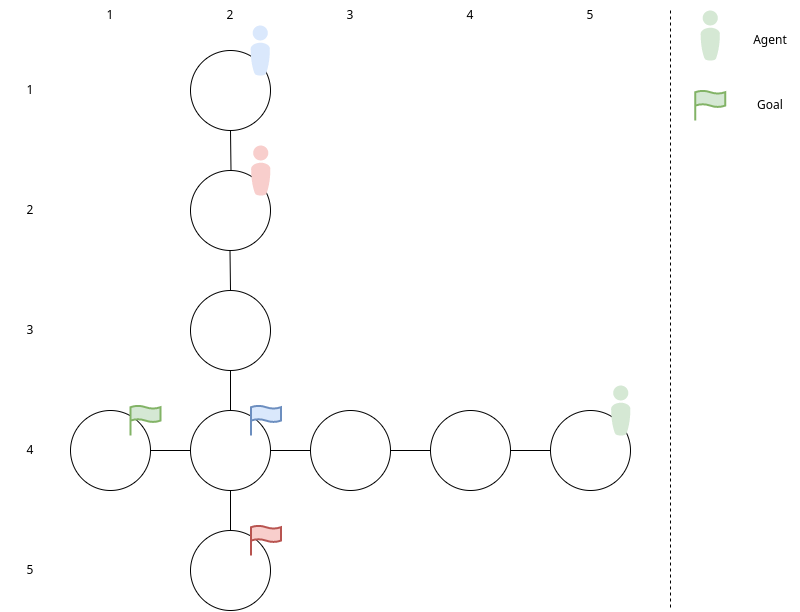
\includegraphics[width=\widthimg]{img/illustrated_instance_format_example.drawio.png}
\end{figure}


\subsubsection{Solver encoding}

As baseline for ASP MAPF solver, we use a MAPF encoding available in the Github framework \textit{asprilo}~\cite{geobotscsangso18a}, we will call it \textbf{base MAPF encoding}. We opted for this encoding due to its simplicity in comprehension and its smooth adaptability to a plan merging approach. In the encoding, we use two primary predicates outlined in the following list~\ref{list:base_mapf_encoding_predicate_explanation}.

\begin{enumerate}\label{list:base_mapf_encoding_predicate_explanation}
    \item \(at(R,P,T)\)  representing the position \(P\) of an agent \(R\) at time step \(T\).
    \item \(move(R,U,V,T)\) representing the movement from vertex \(U\) to vertex \(V\) at time step \(T\).
\end{enumerate}

\begin{minipage}[H]{\linewidth}
\begin{lstlisting}[style=mystyle, caption={Base MAPF encoding}, label={lst:base_mapf_encoding}]
    at(R,P,0) :- start(R,P). |\label{line:init_at}|
    time(1..horizon). |\label{line:init_horizon}|

    {move(R,U,V,T) : edge(U,V)} 1 :- agent(R), time(T). |\label{line:generating_moves}|

    at(R,V,T) :- move(R,_,V,T). |\label{line:generating_at}|
    :- move(R,U,_,T), not at(R,U,T-1). |\label{line:constraining_moves}|
    at(R,V,T) :- |\label{line:waits}|
        at(R,V,T-1), 
        not move(R,V,_,T), 
        time(T). 

    :- { at(R,V,T) }!=1 , agent(R), time(T). |\label{line:one_at_per_t}|

    :- {at(R,V,T) : agent(R)} > 1, vertex(V), time(T). |\label{line:vertex_conflict}|
    :- move(_,U,V,T), move(_,V,U,T), U < V. |\label{line:edge_conflict}|
        
    :- goal(R,V), not at(R,V,horizon). |\label{line:goal_reached}|
\end{lstlisting}
\end{minipage}

In the initial section of encoding~\ref{lst:base_mapf_encoding}, we define, respectively on lines~\ref{line:init_at} and~\ref{line:init_horizon}, the starting positions of each agent and their allocated time using the constant \textit{horizon}.


The rules outlined at line~\ref{line:generating_moves} describe how movement are performed. A possible interpretation could be; for each agent at each available time step and among all available edge going from \(U\) to \(V\), we pick at most one to define one movement at each time.

The rule at line~\ref{line:generating_at} states that if there is a move action is performed by the agent from any location (indicated by \textunderscore) to a different one, the agent is positioned at this destination at this time step.
Then, the rule at line \ref{line:constraining_moves} is a constraint that ensures consistency and coherence in the agent's locations over time. It prevents agents from moving towards a location without having been to the source location at the previous time step. 
Furthermore, the rule at line~\ref{line:waits} specifies that if an agent does not make a move at a specific time step, their location remains the same. 
Finally, the rule \ref{line:one_at_per_t} ensure that an agent is at, at most one defined position at a time.



To conclude the explanation of the base MAPF encoding, the last code section describe how vertex and edge (swap conflict) collisions and goal reaching satisfaction are encoded. First, line~\ref{line:vertex_conflict} outline vertex collision with a constraint rules;  for each vertex, at most one agent can be positioned at a vertex.
Secondly, the rule~\ref{line:edge_conflict} ensure that, no movement from vertex \(U\) to \(V\) and no movement from \(V\) to \(U\) are issued at the same time.
Lastly, the rules~\ref{line:goal_reached} force that, reaching the last possible time step defined by the constant \textit{horizon}, the position of any agent have to be the same as its goal position defined by the predicate \(goal/3\). 

The output of the encoding is the predicate \(at/3\). 
